\documentclass[tikz, border=5pt]{standalone}
\usepackage{amsmath, pgffor}
\usepackage[x11names]{xcolor}
\usetikzlibrary{calc, positioning, decorations.pathmorphing}

\begin{document}
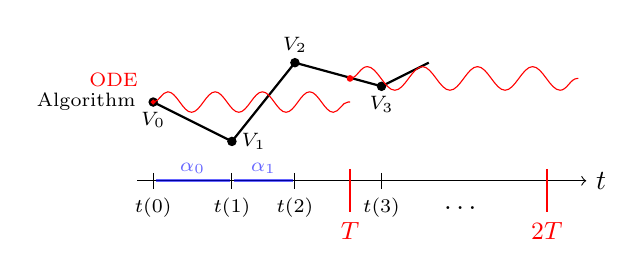
\begin{tikzpicture}

    % Axes
    \draw[->] (-0.2,0) -- (5.5,0) node[right] {$t$};
    \draw (0,0.1) -- (0,-0.1) node[below] {\scriptsize \( t(0) \)};
    \draw (1,0.1) -- (1,-0.1) node[below] {\scriptsize \( t(1) \)};
    \draw (1.8,0.1) -- (1.8,-0.1) node[below] {\scriptsize \( t(2) \)};
    \draw (2.9,0.1) -- (2.9,-0.1) node[below] {\scriptsize \( t(3) \)};
    \node[below] at (3.9,-0.2) {\( \ldots \)};

    % T markings
    \draw[red, thick] (2.5,0.15) -- (2.5,-0.4) node[below] {\small \( T \)};
    \draw[red, thick] (5,0.15) -- (5,-0.4) node[below] {\small \( 2T \)};

    % Segments
    \draw[blue, very thick, opacity=0.6] (0.03,0) -- (1-0.03,0) node[midway, above=-0.05] {\scriptsize \( \alpha_0 \)};
    \draw[blue, very thick, opacity=0.6] (1+0.03,0) -- (1.8-0.03,0) node[midway, above=-0.05] {\scriptsize \( \alpha_1 \)};

    % Graph
    \draw[thick] (0,1) -- (1,0.5) -- (1.8,1.5) -- (2.9,1.2) -- (3.5,1.5);
    \filldraw (0,1) circle (1.5pt) node[below] {\scriptsize \( V_0 \)};
    \filldraw (1,0.5) circle (1.5pt) node[right] {\scriptsize \( V_1 \)};
    \filldraw (1.8,1.5) circle (1.5pt) node[above] {\scriptsize \( V_2 \)};
    \filldraw (2.9,1.2) circle (1.5pt) node[below] {\scriptsize \( V_3 \)};

    % ODE
    \draw[red, decorate, decoration={snake, amplitude=1.3mm, segment length=6mm}] (0,1) -- ++(2.5,0);
    \draw[red, decorate, decoration={snake, amplitude=1.5mm, segment length=7mm}] (2.5,1.3) -- ++(2.9,0);
    \filldraw[red] (0,1) circle (0.7pt);
    \filldraw[red] (2.5,1.3) circle (1pt);

    % Labels
    \node[left=0.1] at (0, 1) {\scriptsize Algorithm};
    \node[red, above left=0.1] at (0, 1) {\scriptsize ODE};

\end{tikzpicture}
\end{document}
